\chapter{Learning on graphs}\label{ml_graphs_chapter}
    In several applications, complex structures such as graphs can represent underlying relationships among data. For example, interactions between people can be modeled with a network, and the knowledge base of Wikipedia is essentially a graph. In general, through the use of graphs it is possible to represent individual features while also providing the structure of such information.
    
    Machine learning techniques have been successfully applied to several Euclidean domains. However, they cannot be directly applied to non-Euclidean structured data. For example, on one hand convolutional neural networks are able to successfully classify images by taking advantage of their grid-like structure. On the other hand, the irregular structure of graphs makes the convolutions not well defined.
    
    In fact, in order to solve this issue, machine learning methods often proceed as follows:
    \begin{enumerate}
        \item They preprocess data by mapping the graph-structured information to a vector space --- i.e., they embed graph-structured data in an Euclidean space.
        \item Then, they apply a traditional technique to learn a function that maps preprocessed data to outputs.
    \end{enumerate}
    Despite some success of these methods, important topological information may get lost during the preprocessing phase: the overall quality of the learning algorithm strongly depends on the intermediate results.
    
    The first graph neural network able to deal directly with data represented in graph domains was proposed in \citeyear{Scarselli} by \citeauthor{Scarselli}: essentially, it learns node representations by propagating neighbor information in an iterative manner until a stable fixed point is reached \cite{Scarselli}\cite{Wu}. However, this technique is very computationally expensive.
    
    \begin{figure}
        \centering
        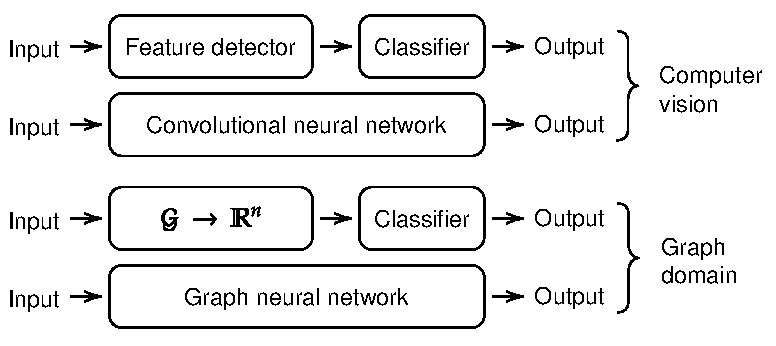
\includegraphics[width=\textwidth]{images/comparison_nn_gnn.pdf}
        \caption{In computer vision, there are several algorithms used to manually extract features from an image (for example, algorithms to detect edges). Such handcrafted features were commonly used by traditional machine learning approaches. On the other hand, modern approaches like convolutional neural networks are able to automatically learn features from data. Similarly, modern graph neural networks do not need a preprocessing stage that maps nodes of a graph to a vector space.}
        \label{comparison_nn_gnn}
    \end{figure}
    
    Since that time, there have been may improvements in graph neural networks. In particular, may studies have focused on developing graph convolutional neural networks --- i.e., convolutional neural networks that are able to learn on irregular lattices such as graphs. These networks, though, require a redefinition of the convolution operation.
    \section{Preliminaries on graph theory}
        Most graph convolutional networks are based on spectral graph theory, which studies the properties of graphs via the eigenvectors and eigenvalues of their associated weighted adjacency matrix and graph Laplacian. Hence it is necessary to present the notation, review how graph spectral domains are defined and point out how operators are generalized to this domain. A complete overview of this field can be found in \cite{Shuman}.
        \subsection{Basic definitions and notations}
            A graph \(\mathcal{G} = \left(\mathcal{V}, \mathcal{E}, W\right)\) consists of a set of vertices \(\mathcal{V}\) (with \(\left|\mathcal{V}\right| = n\)), a set of edges \(\mathcal{E}\) (with \(\left|\mathcal{E}\right| = m\)) and a weighted \(n \times n\) adjacency matrix \(W\).
            \[W_{i,j} =
            \begin{cases}
                \text{Weight of the edge}\ \left(i,j\right) & \text{if}\ \left(i,j\right) \in \mathcal{E} \\
                0 & \text{otherwise}
            \end{cases}\]
            \subsubsection{Domain structure and data on a domain}\label{domainstructure_datadomain}
                It is important to characterize data that can be represented with a graph, and make a distinction between domain structure and data on a domain (see figure \ref{data_on_domain}). Formally:
                \begin{itemize}
                    \item A graph \(\mathcal{G} = \left(\mathcal{V}, \mathcal{E}, W\right)\) represents the structure of the domain. Here only simple graphs are considered --- i.e., graphs without multiple edges or loops). In other words, a graph can represent some relational property according to which the elements of a dataset are connected to each other.
                    \item Node attributes are said to be data on a domain. Formally, an attribute can be thought of as a graph signal: it is a function \(f: \mathcal{V} \rightarrow \mathbb{R}\) defined over the vertices of a graph \(\mathcal{G}\) --- i.e., a function that assign real values to each graph nodes. Vectors \(x \in \mathbb{R}^n\) denote a signal over all the nodes of a graph, where the \(i\)-th component represents the function value at the \(i\)-th vertex in \(\mathcal{V}\).
                \end{itemize}
                
                \begin{figure}
                    \centering
                    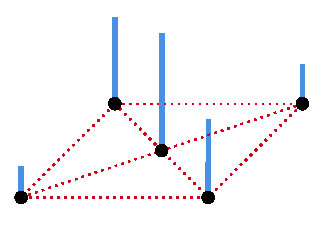
\includegraphics[width=0.5\textwidth]{images/data_on_domain.pdf}
                    \caption{A random positive graph signal on the vertices of a simple graph. The height of each blue bar represents the signal value at the vertex where the bar originates. Instead, the dotted red lines represent the structure of the domain --- i.e., the graph itself.}
                    \label{data_on_domain}
                \end{figure}
            
                Clearly, \textquote{the properties of functions defined on a domain conveys certain information about the domain, and vice-versa, the structure of the domain imposes certain properties on the functions on it} \cite{Bronstein}.
            \subsubsection{Graph Laplacian}
                Given a simple graph \(\mathcal{G}\), its (non-normalized) Laplacian \cite[12]{Chung} is an \(n \times n\) matrix \(L\) defined as:
                \[L = D - W\]
                where \(D\) is the degree matrix --- i.e., a diagonal matrix whose \(i\)-th diagonal element is equal to the sum of the weights of all the edges incident to vertex \(i\) --- and \(W\) is the weighted adjacency matrix.
                
                The graph Laplacian is very important since it links graphs to vector spaces. In other words, it allows to move from discrete to continuous representations.
                
                It can be proven that \(L\) is a positive semi-definite matrix (\(x^T L x > 0\) for all non-zero \(x \in \mathbb{R}^n\)). The Laplacian is also a symmetric matrix, hence it admits a set \(n\) orthonormal eigenvectors, denoted by \(\Phi = \left(\phi_1, \phi_2, \dots, \phi_n\right)\)\footnote{There is not necessarily a unique set of eigenvectors, but one can assume that a set of eigenvectors is chosen and fixed.}. These eigenvectors have associated real, non-negative eigenvalues \(\lambda_1, \lambda_2, \dots, \lambda_n\) (which are usually called the spectrum of the Laplacian \cite[4]{Chung}).
                
                The normalized graph Laplacian can be obtained by normalizing each weight \(W_{i,j}\) by a factor \(\frac{1}{\sqrt{d_i \cdot d_j}}\), where \(d_i = D_{i,i}\). It is equivalently defined as:
                \[\tilde{L} = D^{-\frac{1}{2}}LD^{-\frac{1}{2}} = I - D^{-\frac{1}{2}}WD^{-\frac{1}{2}}\]
        \subsection{Spectral graph theory}
            Spectral graph theory studies the properties of graphs via the eigenvectors and eigenvalues of their associated weighted adjacency matrix and graph Laplacian. It enables the processing and analysis of signals that lie on structured but irregular domains such as graphs: in order to do so, one must generalize classical signal processing concepts, tools and methods on graphs.
            \subsubsection{Graph Fourier transform}
                The classical Fourier transform is a complex-valued representation of a function of time --- i.e., a signal --- in the frequency domain\footnote{The Fourier transform is not limited to functions of time, but the domain of the original function is commonly referred to as the time domain.}. In other words, it expresses a signal in term of the frequencies of the waves that make up the signal. Specifically, the Fourier transform describes how much any given frequency is present in the original function. Formally:
                \[\hat{f}\left(\xi\right) = \left\langle f, e^{2 \pi i \xi t}\right\rangle =  \int_{-\infty}^{+\infty}f\left(t\right)e^{-2 \pi i \xi t}dt\]
                where \(\xi\) represents frequency and \(t\) represents time. While the Fourier transform maps a function to a set of complex numbers representing sinusoidal coefficients, the inverse Fourier transform maps in the other direction.
                
                Fourier transform is important because a lot of problems that are very difficult to solve directly become easy in the frequency domain. In particular, operations performed in one domain have corresponding operations in the other domain, which are sometimes easier to perform: for example, one can get the Fourier transform, perform the desired operations in the frequency domain and then transform back the result to the time domain.
                
                The graph Fourier transform \(\hat{f}\) of a signal \(f \in \mathbb{R}^n\) defined over the vertices of \(\mathcal{G}\) is defined as an expansion of \(f\) in terms of the eigenvectors of the graph Laplacian:
                \[\hat{f}\left(\lambda_l\right) = \left\langle f, \phi_l \right\rangle = \sum_{i=1}^{n}f\left(i\right)\phi_l\left(i\right)\]
                In matrix form:
                \[\hat{f} = \Phi^T f\]
                
                \begin{figure}
                    \centering
                    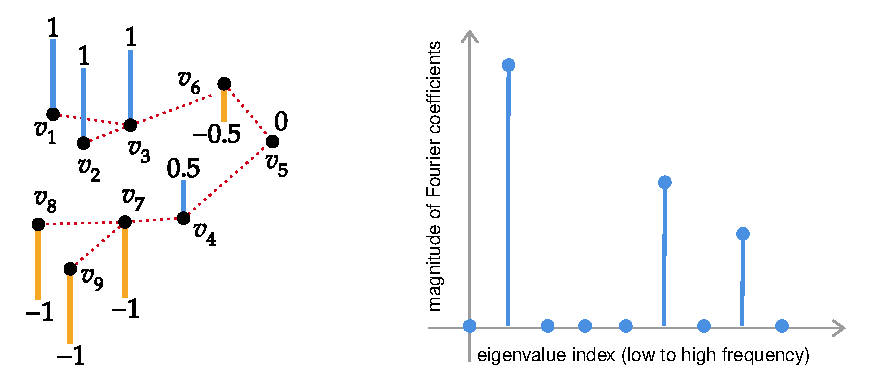
\includegraphics[width=\textwidth]{images/spectral_domain.pdf}
                    \caption{A signal on the graph and its Fourier coefficients in the graph spectral domain.}
                    \label{spectral_domain}
                \end{figure}
                
                The graph Fourier transform allows to represent a signal in the graph spectral domain (see figure \ref{spectral_domain}). Signals in the spectral domain are often referred to as kernels. Also, in signal processing on graphs, the eigenvalues \(\lambda_1, \lambda_2, \dots, \lambda_n\) of \(L\) are called graph frequencies and they form the spectrum of the graph. The\(l\)-th eigenvector \(\phi_l\) related to the eigenvalue \(\lambda_l\) is called frequency component corresponding to the \(l\)-th frequency \cite{Sandryhaila}.
            \subsubsection{Convolution}
                Convolution is one of those operations which are much more manageable in the frequency domain. Specifically, it simply corresponds to ordinary multiplication in the frequency domain. In other words, one can perform a convolution by taking the Fourier transform of both functions, multiplying the results, and then performing an inverse Fourier transform. Formally:
                \[f \star g = \widehat{\hat{f} \cdot \hat{g}}\]
                
                The convolution operation can be generalized to signals on graphs by using the Laplacian eigenvectors \(\phi_1, \phi_2, \dots, \phi_n\). Here is one way to do it \cite{ShumanWindowed}:
                \[\left[f \star g\right]\left(i\right) = \sum_{l=1}^{n}\hat{f}\left(\lambda_l\right)\cdot\hat{g}\left(\lambda_l\right)\cdot\phi_l\left(i\right)\]
                Such definition enforces the property that convolution in the vertex (time) domain is equivalent to multiplication in the graph spectral domain. More generally, it can be expressed in matrix notation \cite{Defferrard}:
                \[f \star g = \Phi \Lambda \Phi^T f\]
                where \(\Lambda = diag\left(\hat{g}\left(\lambda_1\right), \hat{g}\left(\lambda_2\right), \dots, \hat{g}\left(\lambda_n\right)\right)\)
        \subsection{Graph coarsening}
            Often, in the graph world data come in big sizes. On one hand this means richer training sets, but on the other hand big graphs cause non-trivial computational problems, especially when one try to apply machine learning techniques to them.
            
            A common idea is to coarse a graph and get a reduced approximation of the original one, hopefully at a low cost. The final solution can then be found (and possibly refined) on such a reduced graph. However, it is important for the coarse graph to be a good substitute of the original graph: it must preserves the global structure and only lacks in details. Graph coarsening is the equivalent of pooling when dealing with graphs.
            
            The process of transforming a graph \(\mathcal{G} = \left(\mathcal{V}, \mathcal{E}, W\right)\) into a coarser graph \(\mathcal{G}_{reduced} = \left(\mathcal{V}_{reduced}, \mathcal{E}_{reduced}, W_{reduced}\right)\) with fewer vertices and edges --- while also preserving some global properties --- can be split in two related subtasks \cite{Shuman}:
            \begin{enumerate}
                \item Identifying a reduced set of vertices \(\mathcal{V}_{reduced}\). Such task is called graph sub-sampling when the additional constraint \(\mathcal{V}_{reduced} \subset \mathcal{V}\) is imposed.
                \item Assigning edges \(\mathcal{E}_{reduced}\) and weights \(W_{reduced}\), and connecting the new set of vertices.
            \end{enumerate}
            Several graph coarsening techniques have been proposed (\cite{Lafon} and \cite{Defferrard} to mention a few), but the problem is difficult and this is still an open question.
    \section{Spectral-domain geometric learning}\label{spectralgeometriclearning}
        Geometric learning is the field that aims to build neural networks that can learn from non-Euclidean data, such as graphs. In particular, most of these methods use spectral graph theory.
        \subsection{General spectral graph convolutional neural networks}
            Spectral graph convolutional neural networks share their architecture with convolutional neural networks used in Euclidean domains. In particular, they are a combination of convolutional layers --- with filters defined on graphs --- and pooling layers\footnote{Pooling layers are usually not used when the goal is to classify the nodes of a graph.} --- which implements a graph coarsening process (see figure \ref{architecture_CNN_graphs}) \cite{Defferrard}.
            
            \begin{figure}
                \centering
                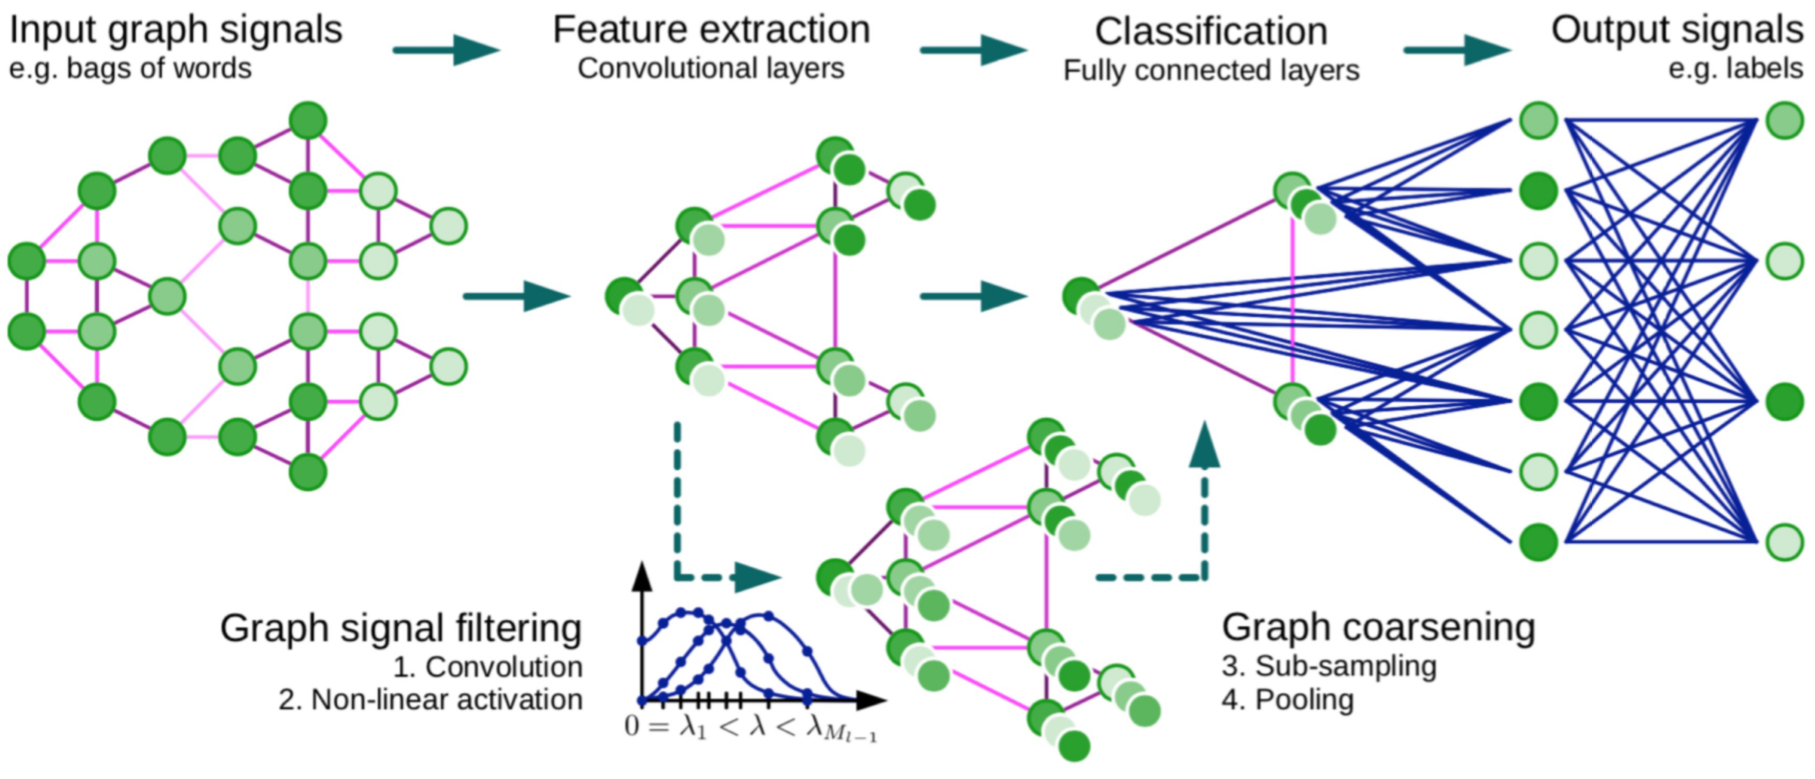
\includegraphics[width=\textwidth]{images/architecture_CNN_graphs.PNG}
                \caption{Architecture of a general spectral graph convolutional neural network \cite{Defferrard}.}
                \label{architecture_CNN_graphs}
            \end{figure}
            
            The complexity of the convolution operation --- i.e., the number of parameters in the convolutional layer --- is directly influenced by the design of the spectral filter and by the spectrum itself.
        \subsection{Graph convolutional networks}\label{gcn}
            \citeauthor{Kipf}, some of the pioneers in this field, published in \citeyear{Kipf} a very important paper \cite{Kipf} in which the present graph convolutional networks: they start from the framework of spectral convolutions and then they introduce some simplifications to improve training times.
            
            Computing the convolution as \(f \star g = \Phi \Lambda \Phi^T f\) and computing the eigenvalues of a large graph is computationally expensive \cite{Kipf}. In order to solve this problem, they approximated the computation of the convolution with an efficient numerical implementation:
            \[f \star g \approx \theta \left(I - D^{-\frac{1}{2}} W D^{-\frac{1}{2}}\right)f\]
            where \(D\) is the diagonal node degree matrix.
            
            Moreover, they introduced a re-normalization trick, since repeated applications of the previous equation can lead to numerical instabilities and gradient vanishing when dealing with deep neural networks:
            \[I - D^{-\frac{1}{2}} A D^{-\frac{1}{2}} \rightarrow \tilde{D}^{-\frac{1}{2}} \tilde{W} \tilde{D}^{-\frac{1}{2}}\]
            with \(\tilde{W} = W + I\) and \(\tilde{D}_{i,i} = \sum_{j}\tilde{W}_{i,j}\).
            
            In their paper, \citeauthor{Kipf} experimented with graph convolutional networks and found out that they are \textquote{capable of encoding both graph structure and node features in a way useful for semi-supervised classification} \cite{Kipf}. Also, the proposed method outperformed many others by a great margin, while being computationally efficient. This method implicitly assumes locality though --- i.e., the classification of a node depends only on the neighborhood. Therefore, a network with \(K\) layers is needed if one wants to extend this dependence to the \(K\)-th order neighborhood. 